\chapter*{Ejercicio 11}
\section*{Caja con tapa superior}

11. De un pedazo rectangular de cartón de 6 ft pot 10 ft se va a fabricar \textbf{\textit{una caja con tapa superior}} doblando a lo largo de las líneas punteadas, cortando cuatro cuadrados del mismo tamaño (véase la figura 1) y plegando dentro de la caja las dos pestañas extras.
\newline
\begin{center}
     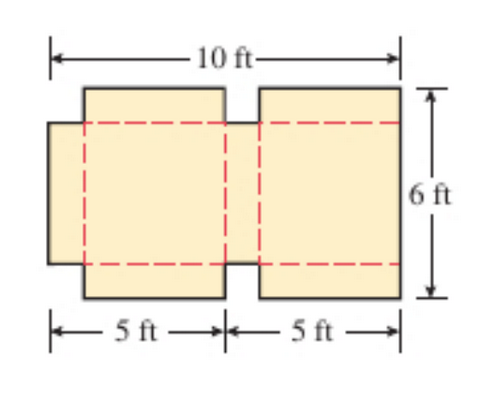
\includegraphics[width=5cm]{recursos/Caja_doc_tarea.png}\par
\end{center}

\textbf{a)} Hallar una fórmula que exprese el volumen V de la caja como función de la longitud x de los lados de los cuadrados que se cortan.\\
\[
V = (largo)(ancho)(alto)
\]
\begin{itemize}
        \item $largo = 5 -x$
        \item $ancho = 6 -2x$
        \item $alto = x$
    \end{itemize}
\[
V(x) = (5-x)(6-2x)(x)
\]
\[
V(x) = (30-10x-6x+2x^{2})(x)
\]
\[
V(x) = (30-16x+2x^{2})(x)
\]
\[
V(x) = 2x^{3}-16x^{2}+30x 
\]
\begin{center}
    Fórmula para el volumen en función de x: \underline{ $V(x) = 2x^{3}-16x^{2}+30x $ ft³} 
\end{center} 

\textbf{b)} Describa, mediante una desigualdad que acote los posibles valores de x, el dominio de definición de a función V = V (x) del inciso anterior. \\
\newline
Dominio Natural de V(x): $R$ \\
Dominio de Definición de V(x): $0 < x < 3$
\begin{itemize}
    \item x debe ser mayor de 0 para que pueda doblar y formar la caja. $x > 0$
    \item x debe ser menor de 3 o no podría haber 2x en el lado de 6 ft. $x < 3$
\end{itemize}
\begin{center}
    Dom. Definición: \underline{$0 < x < 3$}
\end{center}



\textbf{c)} Usar la gráfica de V = V(x) para dar valores aproximados de las dmonsiones de la caja de máximo volumen.
\begin{center}
     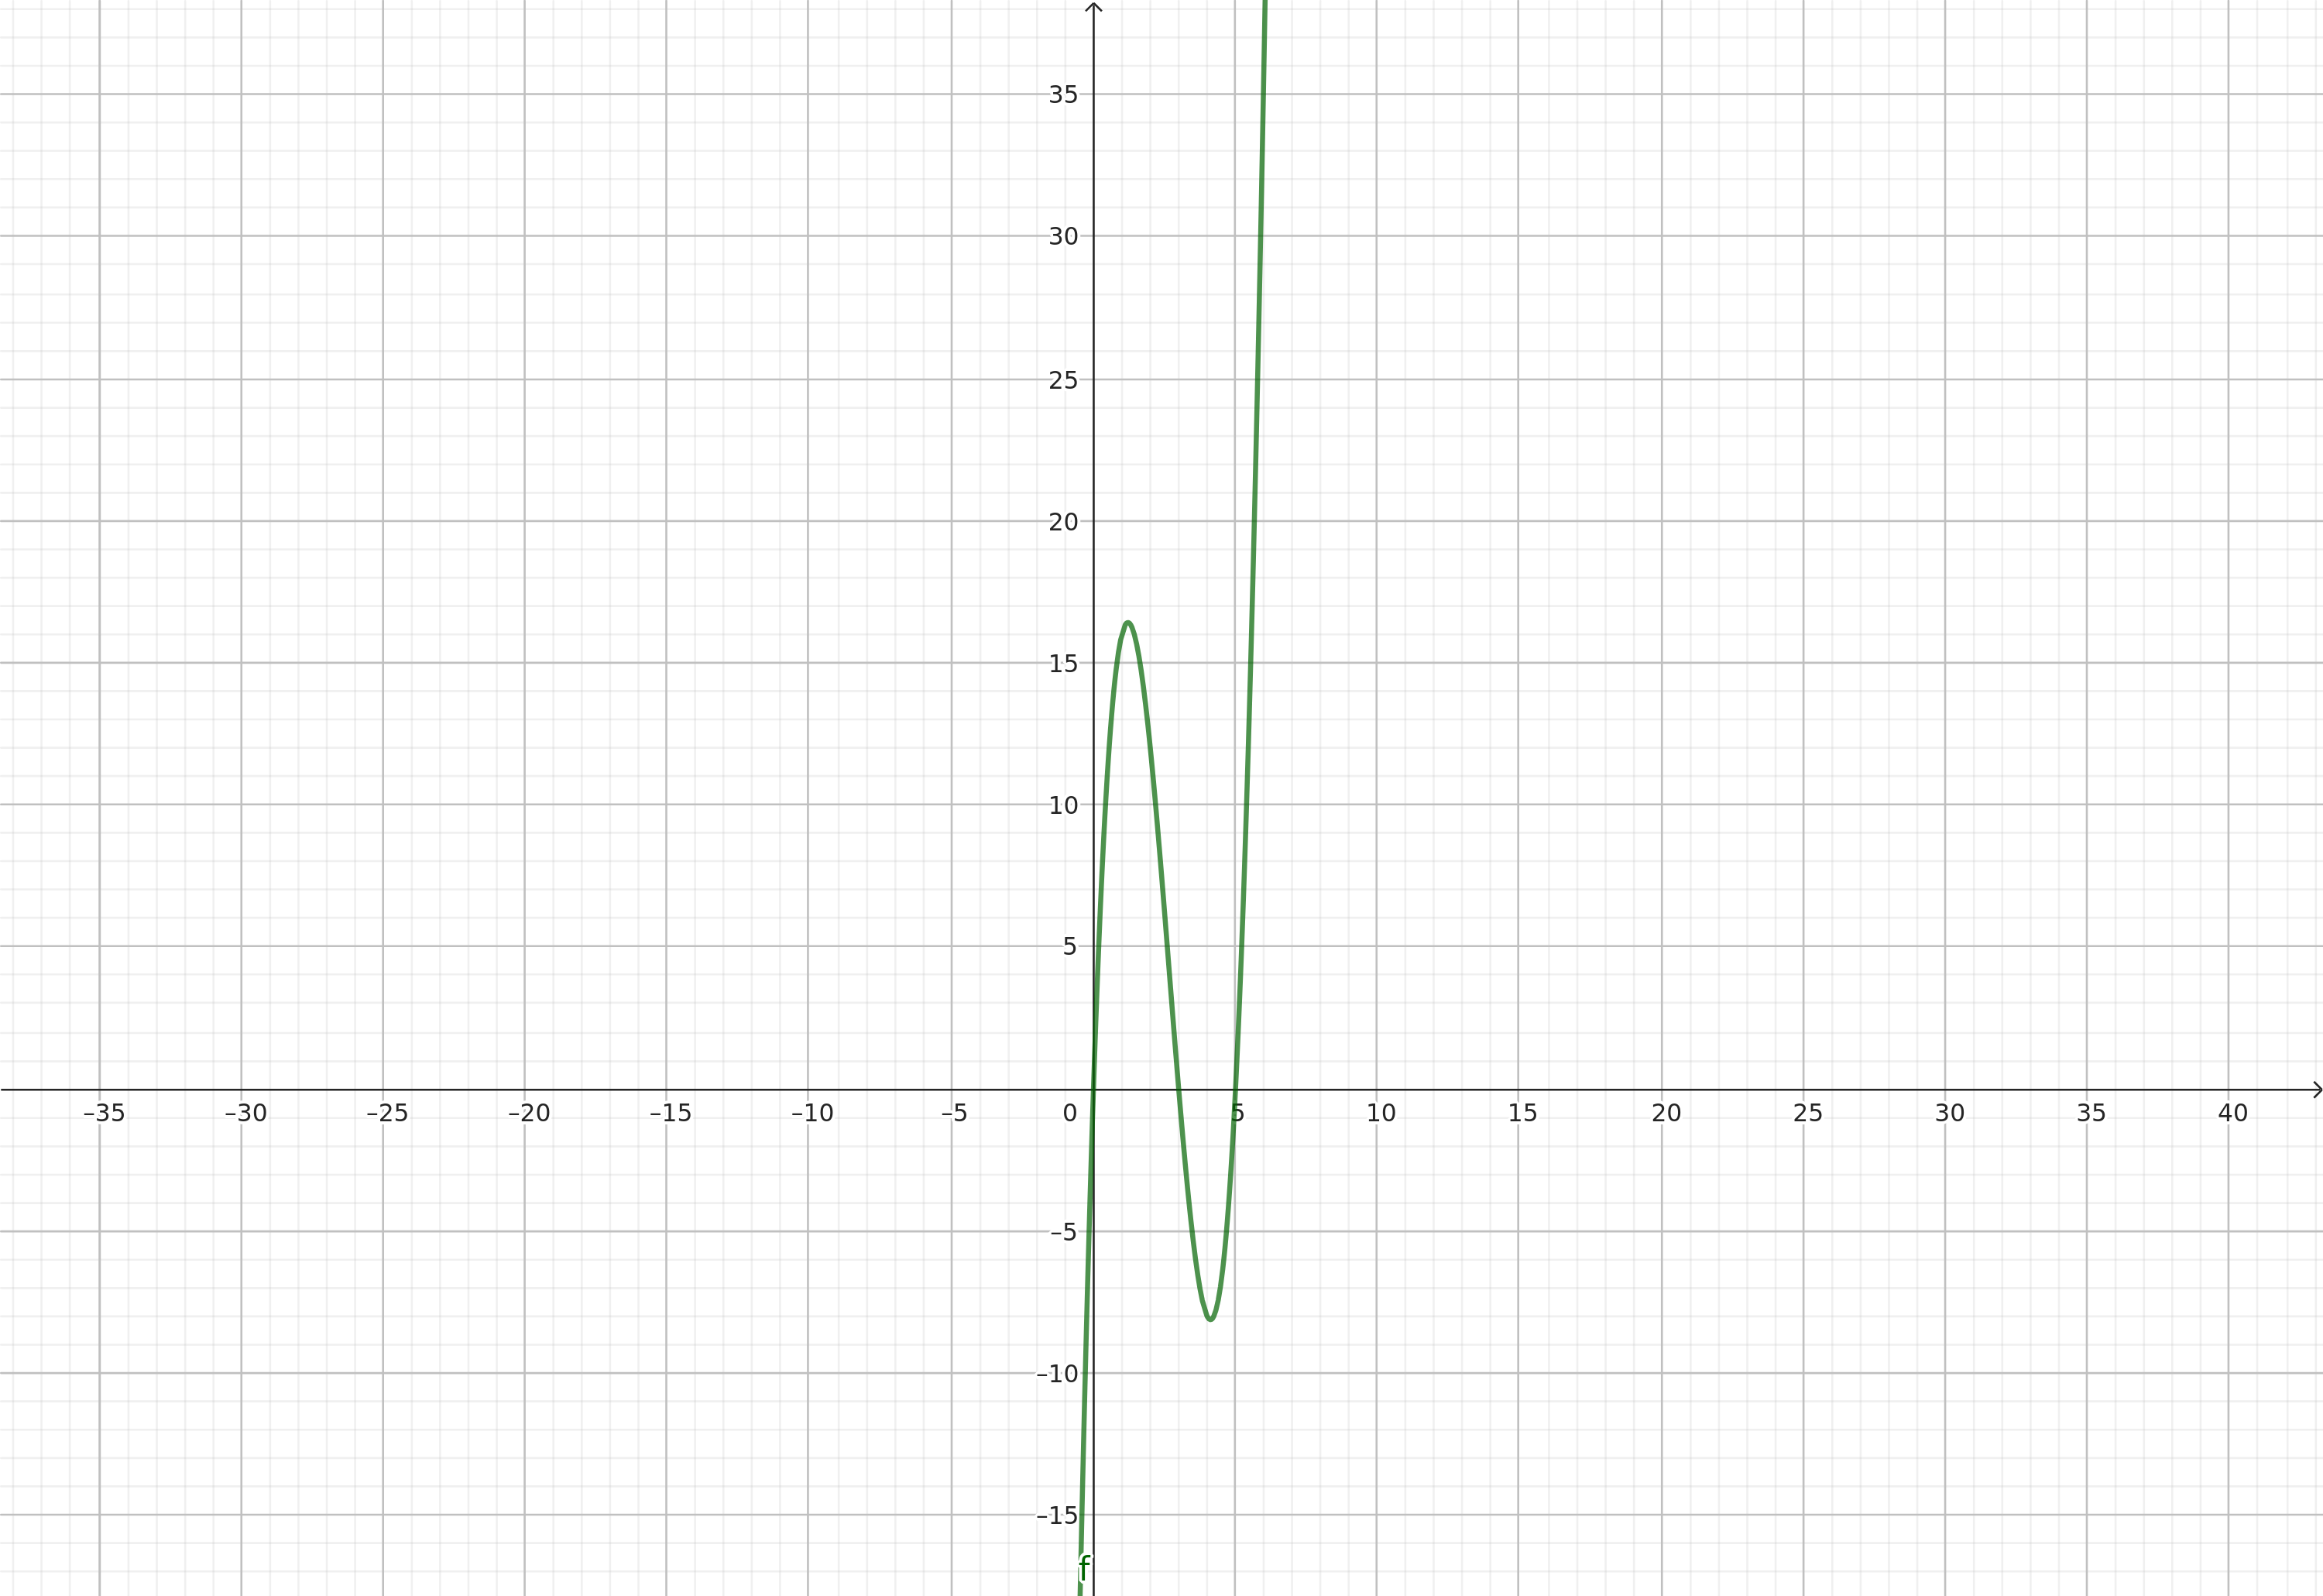
\includegraphics[width=9cm]{recursos/Grafic_caja.png}\par
     Gráfica de $V(x) = 2x^{3}-16x^{2}+30x $
\end{center}
\par
\begin{center}
     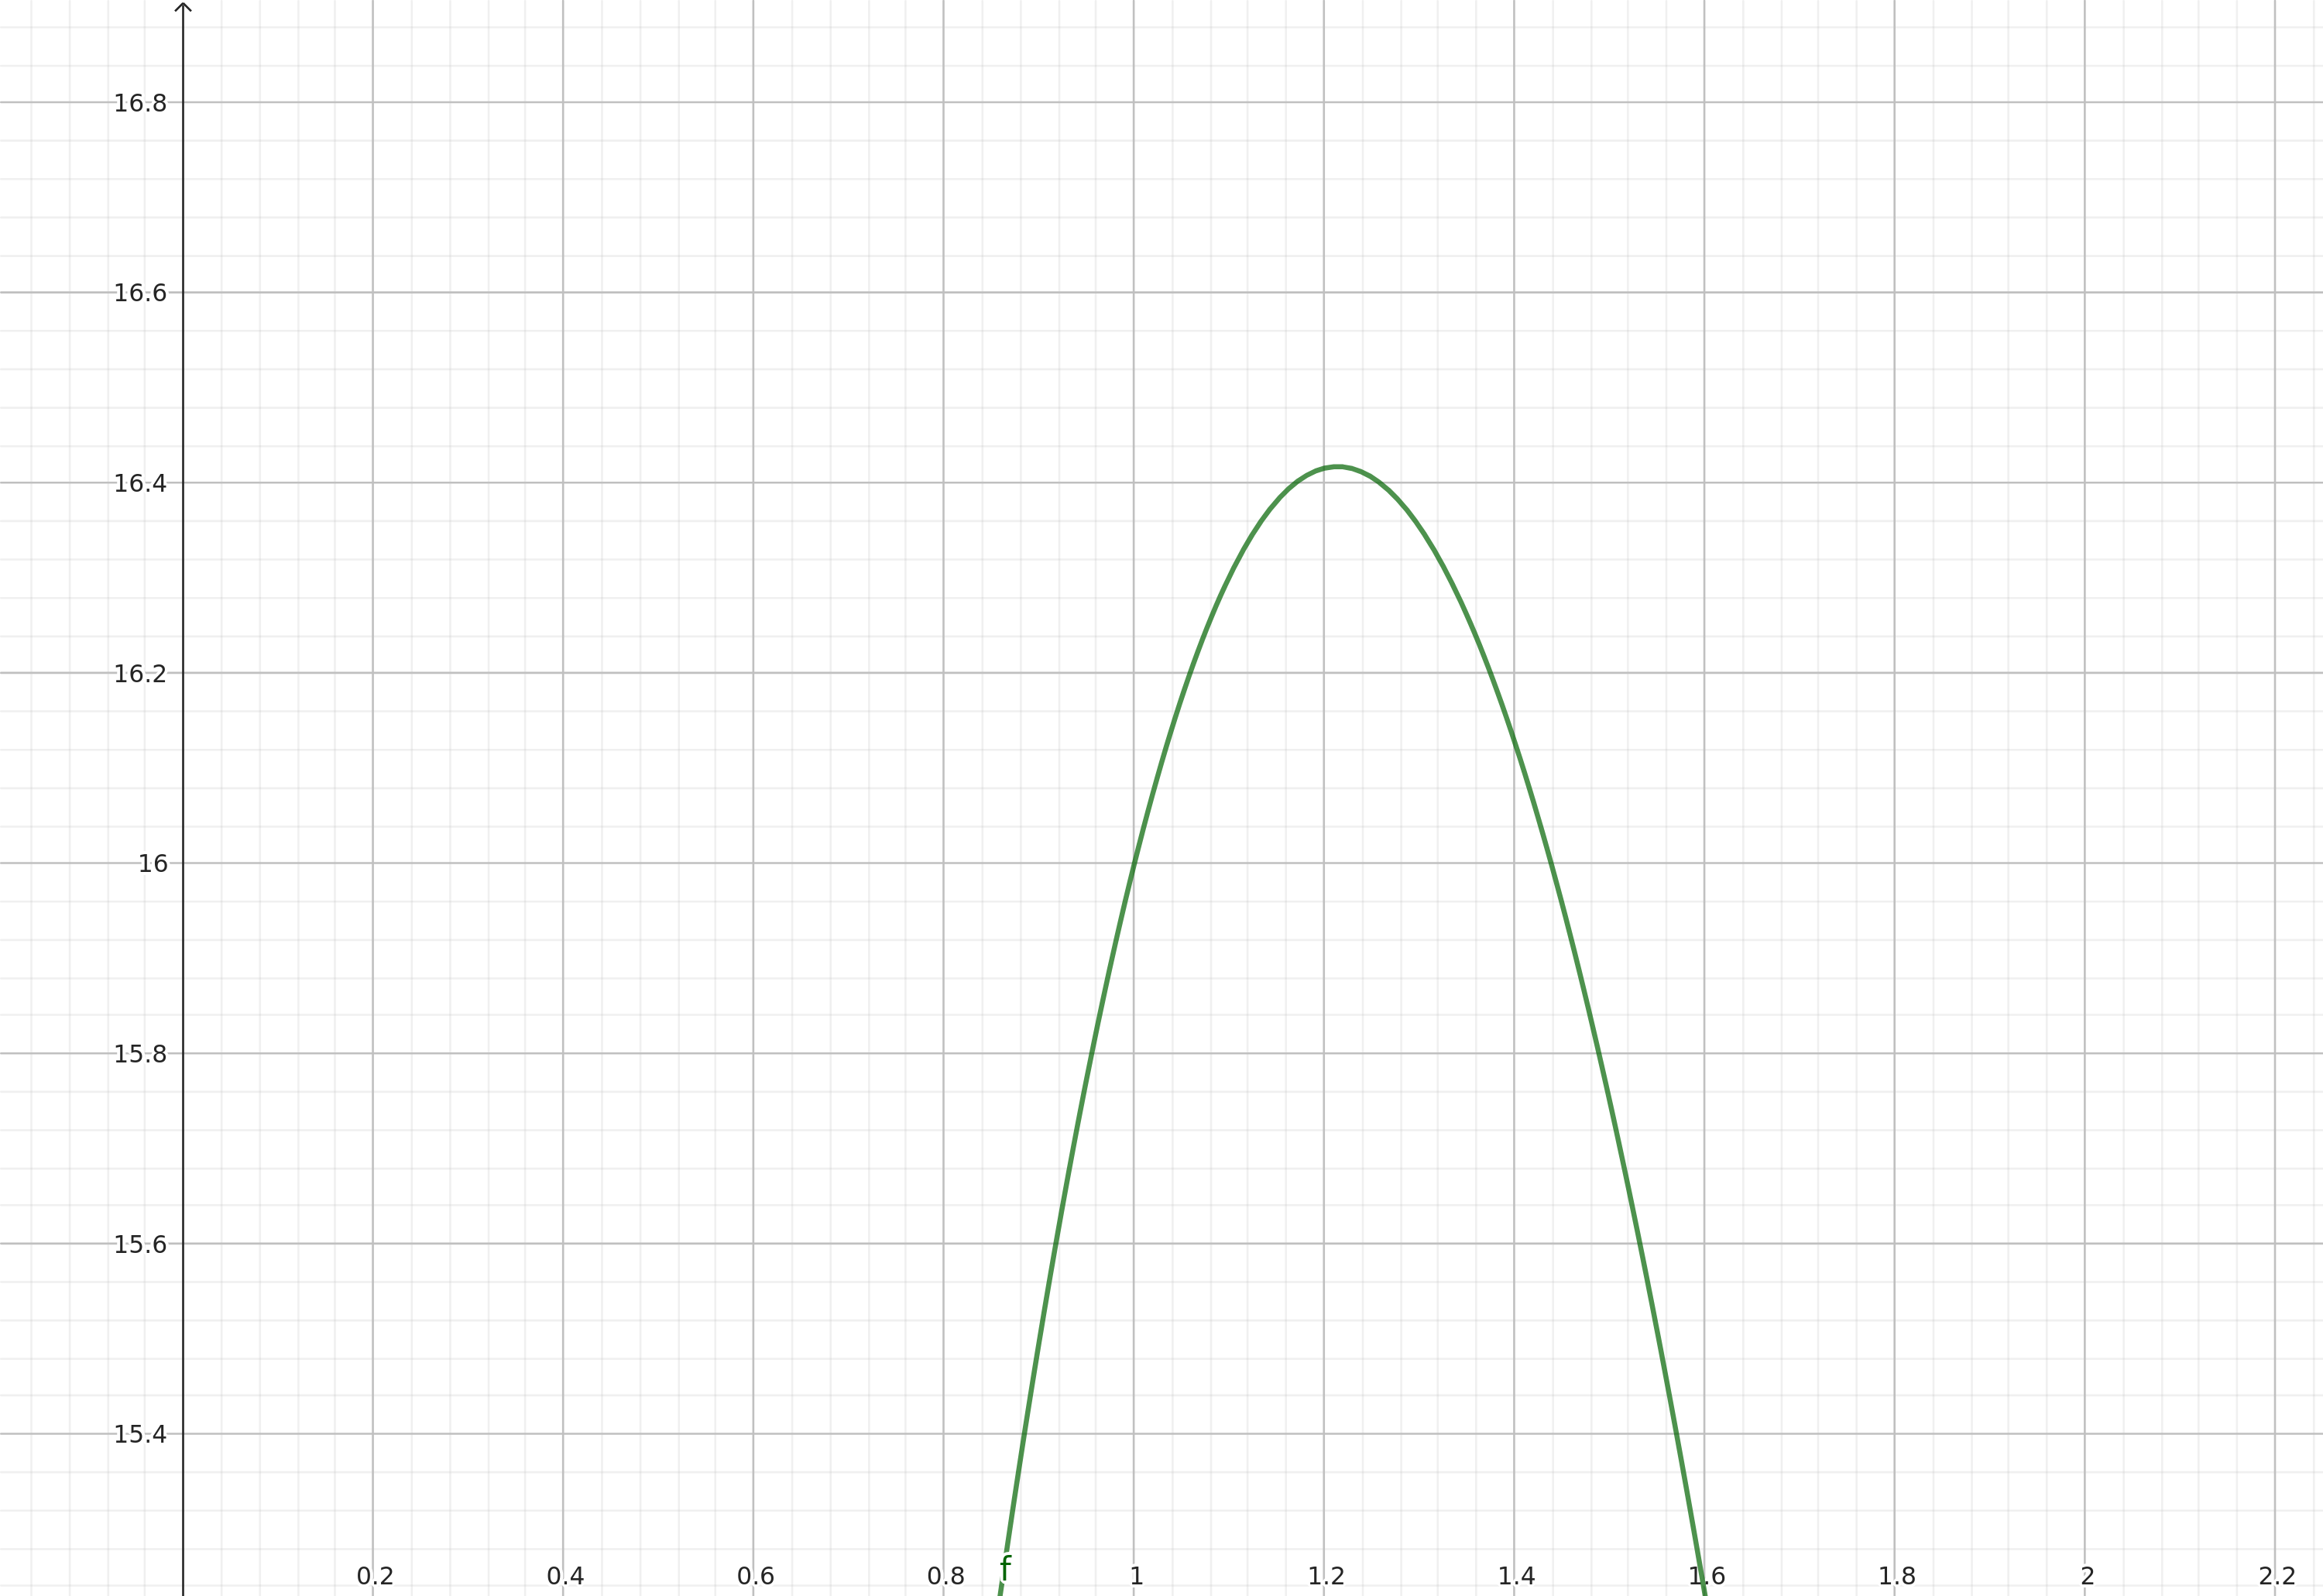
\includegraphics[width=9cm]{recursos/Problema_caja3.png}\par
     Valores Máximos que toma el volumen: \\
     Cuando $x$ se aproxima a 1.2137\\
     $Vol. Max. \approx 16.4176  ft^{3}$
\end{center}
